\chapter{Plans}\label{C:future}

\section{Design}
As I'm building the tool as a web based system, I have been forced to use a client server model.
Use of web based systems leads to some security concerns regarding access control and system robustness.

Using web based technologies has the advantage of tapping into significant existing work in visualisation libraries 
and remote database access, see Section \ref{tools} for details.

Significant work remains to be done on the database schema for storing SSHD log entries, These entries are highly structured, which allows for a relatively simple parser to break down into usable form. As existing designs call for a raw text view to accompany the main visual components (see Section \ref{screen_design}) I propose to store the raw log entry as a text field  within the database. Some design work is required to describe a storage mechanism for information about individual users and network structure. The minimum information required would be typical access times and locations for users and server names, locations and uses for machines. I do not forsee significant difficulties in designing a storage layout for this data.

Design of server side code and functions remains to be carried out, though I plan to perform the majority of data processing server side, due to concerns about javascript and browser performance when hundreds of thousands to millions of elements are being manipulated. 

\section{Security Concerns}
As I'm building the tool as a client server model, accessed through the browser
there are several security concerns to be considered in a deployment of the system.
The database will contain a significant amount of privileged information about network security
such as machine names and addresses, valid account names, and authentication methods used in the system.

This data would be extremely useful to malicious users or outside intruders. 
This leads to a need to ensure that access to this database is controlled through a robust authentication system.
Ideally the web server hosting the tool should not be accessible to the outside world at all. Within the organisation's private network access should be restricted tightly to only those users with a definite need to have access. 
Secured connections must be used for all communication between client and server to limit the opportunity for malicious individuals to snoop on the data in transit.

Security of the serverside code will be considered from the beginning of the design and implementation process
as this code must be able to resist any malicious access attempts. Through input sanitation and bounds checking should serve to close the majority of possible vulnerabilities.

Client side code contains no data, and so is significantly less critical to secure, as the database systems should deny access without valid credentials. Ideally host based authentication could be used. However, implementing a robust access control scheme does not fit within the scope of this project, and will be left for future development.

\section{Implementation}

Implementation of the tool remains to be started, this along with evaluation comprise the majority of remaining work to be performed.
I will be using a github repository for version control and backup purposes.

\subsection{Tools and Languages}\label{tools}

As I have elected to use a client server model with the client residing in a web browser a suitable server side language must be chosen to allow database connectivity. I am largely unaware of the strengths and weaknesses of various server side languages. Further research is needed to decide between the various possibilities. Java appears on the surface to be a strong contender due to language familiarity and strong tool support through eclipse. Tomcat provides a solid framework for interfacing web requests with java code.
Many other languages remain, such as perl, php, and ruby or even serverside javascript. Each of these languages requires learning a new language effectively from scratch, this is a significant time cost on a short project. 

\subsection{Testing}
Automated testing of user interfaces remains problematic, with many tools suffering from severe fragility where UI layout is modified. In most testing libraries, mous interaction is recorded at test design, then played back artificially on execution, This causes severe fragility as if a control or button moves the recorded mouse movements will miss the button, causing test failures. Further research is needed to find a testing library suitable for testing, however the test automation tool created by Dojo appears useful \cite{dojo2013test}.

\section{Timeline}

I will be taking a couple of days as a complete break from university work following my exams on the 15th and 17th of June, with work on the project resuming on 19th June. Figure \ref{gantt} shows a Gantt chart breaking down my plans for the remainder of the work to be completed.  I expect to be done implementing the tool early in second trimester, with at least a month left after evaluation is complete to write up my final report before end of teaching trimester 2.
  
\begin{figure}[tbh]
\fbox{\parbox[b]{.99\linewidth}{
\vskip 0.5cm
\centering 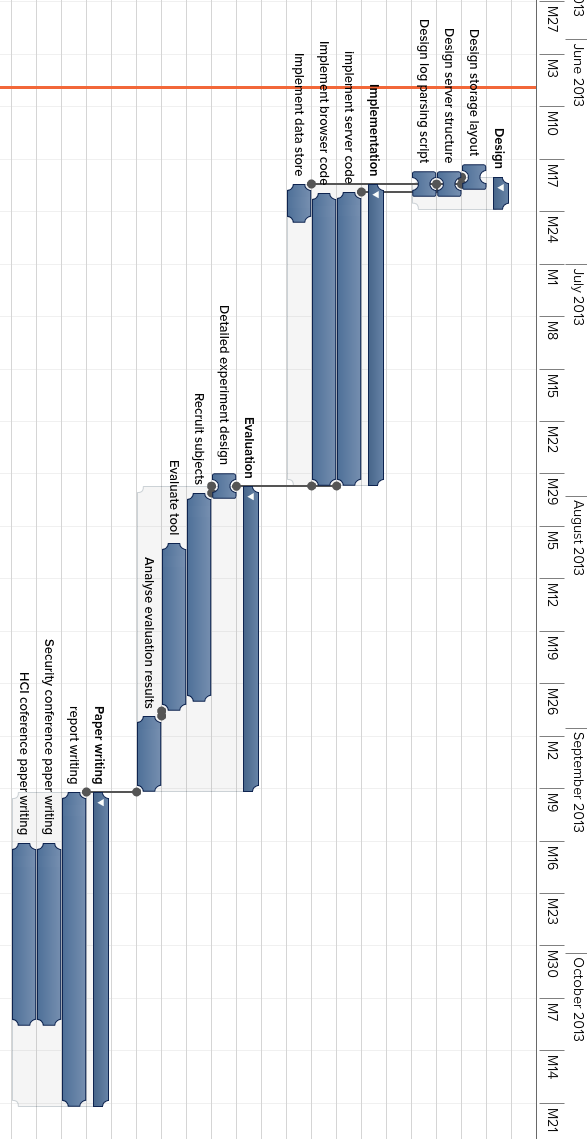
\includegraphics[scale=0.75]{gantt.png}
\vskip 0.5cm}}
\caption{\protect\label{gantt}Gantt chart showing breakdown of future work into major sections. The design group is all sub day tasks.}
\end{figure}

\subsection{Risks}

Several notable risks remain to this project.
\begin{description}
\item[Languages:] Learning a new programming language always carries risks of unexpected setbacks or difficulties in completing tasks due to lack of familiarity with language features and libraries. This can be mitigated through choosing languages appropriate to the tasks, ideally already well known languages. 
\item[Experiment Participants:] User evaluations always carry an element of risk in recruiting a suitable number of participants in the time available to complete the study. This can be mitigated through an early start to the recruitment process, and well chosen incentives. 
\item[Ethics approval:] User experiments carry an element of risk, as if ethics approval is delayed significantly, this will cause severe dislocation to the planned timeline, which may limit the evaluation after approval is gained. This is unlikely as approval has been sought already, and the application is before the committee.  
\end{description}